% capítulo 1 - introdução
% ------------------------------
% estrutura do capítulo
% 1. Introdução
% 1.1 Tema 
%     1.1.1 Delimitação do tema
% 1.2 Problemas e premissas
% 1.3 Objetivos
%     1.3.1 Objetivo geral 
%     1.3.2 Objetivos específicos
% 1.4 Justificativa
% 1.5 Estrutura do trabalho
% -------------------------------

% 1 ------------- introdução
\chapter{Introdução}\label{cap:introducao}


A robótica é uma área em constante evolução, marcada por avanços significativos ao longo de sua história, que trouxeram transformações não apenas no âmbito econômico, mas também nas esferas social, científica e tecnológica. Desde seus primórdios na indústria até o surgimento dos mais recentes robôs colaborativos, essa tecnologia tem permeado cada vez mais nosso cotidiano.

Segundo estimativas feitas pela \emph{Interact Analysis}, espera-se que mais de 150.000 robôs de coleta - ou \emph{picking robots}, em inglês - sejam instalados até o final da década \cite{Wessling2023}. E no lado econômico, as projeções da empresa de consultoria \textit{Boston Consulting Group} apontam que o mercado de robótica cresça de US\$ 25 bilhões em 2021 e para até US\$ 260 bilhões em 2030 \cite{Carmen2021}.

Tais indicadores demonstram a importância crescente da robótica na economia global. No entanto, os avanços recentes vão além da produção industrial, chegando a áreas como a saúde, transporte e serviços. Robôs colaborativos, exoesqueletos e drones autônomos são exemplos de tecnologias robóticas recentes que têm o potencial de impactar positivamente esses setores.

Com a crescente demanda por soluções autônomas e eficientes em diferentes setores, a pesquisa sobre navegação natural em robôs móveis autônomos tem se tornado cada vez mais relevante. Ao desenvolver o AMR Frederico, estamos contribuindo não apenas para a competição de \emph{Robomagellan}, mas também para a evolução da robótica como todo. A aplicação de tecnologias avançadas tem o potencial para impactar positivamente diversos setores, desde a indústria, até a saúde e o transporte, melhorando a precisão, eficiência e segurança em diferentes operações.

% 1.1 ----------- tema 
\section{\textbf{Tema}}
% o tema é AMR
Os Veículos Guiados Automaticamente (AGV) foram uma das primeiras formas de automação em ambientes industriais. Originalmente introduzidos nas décadas de 1950 e 1960, os AGVs eram projetados para seguir trajetórias fixas, frequentemente utilizando trilhos, fitas magnéticas ou guias visuais para navegar em ambientes controlados, como fábricas e armazéns. Com o passar do tempo, esses sistemas evoluíram e, nas últimas décadas, desempenharam um papel fundamental na automação industrial, especialmente na movimentação de materiais pesados {Ullrich2023}.

\begin{figure}
    \centering
    \captionsetup{justification=centering}
    \caption{\small Um dos primeiros modelos de AGV lançado nos EUA em 1954}
    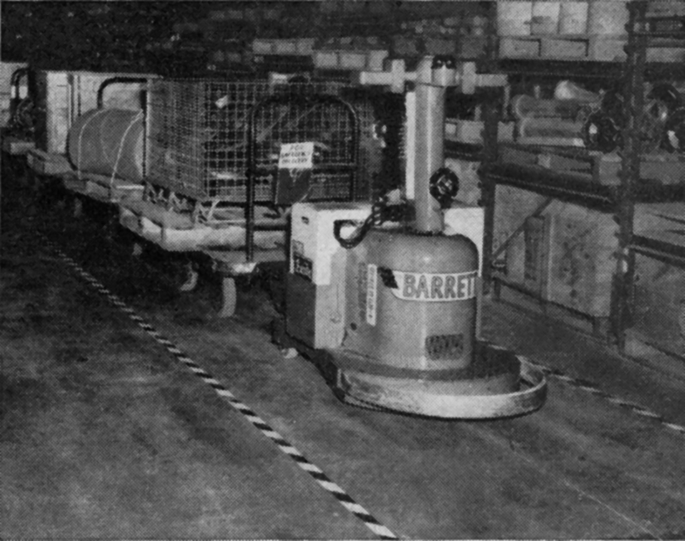
\includegraphics[width=0.5\textwidth]{imagens/AGV-1950.png}
    
    {\small Fonte: \cite{Ullrich2023}}
\end{figure}

O avanço da tecnologia trouxe aprimoramentos significativos para os AGVs. Sensores mais avançados têm sido incorporados, permitindo um nível mais alto de percepção e interação com o ambiente. Além disso, a capacidade de conexão e comunicação entre robôs tem permitido a criação de uma central de controle centralizado, ampliando as possibilidades de coordenação e eficiência dentro dos ambientes industriais. 

Mas além da evolução de AGVs, essa evolução tecnológica permite a entrada de outro ator na cena, os Robôs Móveis Autônomos, ou \emph{Autonomous Mobile Robots} (AMR), em inglês. Agora podemos substituir robôs baseados em orientação física, limitado a navegar em um ambiente pré-definido em um caminho pré-definido, para um que seja totalmente autônomo. 

\begin{quote} % citação longa direta
    \setlength{\leftskip}{4cm} % Recuo de 4cm da margem esquerda
    \setlength{\rightskip}{0cm} % Sem recuo na margem direita
    \footnotesize % Tamanho da fonte 10pt
    \setlength{\parskip}{1em} % Espaçamento entre os parágrafos (1em ou qualquer outro valor desejado)
    \setlength{\parindent}{0cm} % Remover indentação dos parágrafos    

    Um AMR é capaz de navegar em um ambiente imprevisível. Os AMRs podem detectar os parâmetros do ambiente e criar um modelo do ambiente, localizando-se neste modelo. Esse comportamento permite que o AMR crie um plano de navegação e otimize esse plano por meio de um algoritmo de planejamento especial, [...] além disso, pode criar um mapa do ambiente usando dados dos sensores e se localizar no mapa ao mesmo tempo. \cite[p.1, tradução nossa]{Murat2017}    

\end{quote}

Os robôs móveis autônomos (AMR) representam uma das áreas mais empolgantes da robótica contemporânea, são sistemas capazes de navegar em ambientes complexos e interagir com seu entorno usando sensores e atuadores. Eles oferecem uma gama de aplicações práticas, desde manufatura até exploração espacial. No cerne desses sistemas, a navegação autônoma desempenha um papel crucial.


% 1.1.1 --------- delimitação do tema 
\subsection{Delimitação do tema}

Nesta dissertação estudaremos os aspectos de implementação da navegação natural em robôs móveis autônomos. O objeto de estudo deste trabalho será o AMR Frederico, desenvolvido por mim e minha equipe, composta por Guilherme, Pedro, João, João A, Amora, Caio e Ale, no projeto de extensão \emph{O PROJETO} desde 2022. 

\begin{figure}[h]
    \centering
    \captionsetup{justification=centering}
    \caption{\small AMR Frederico}
    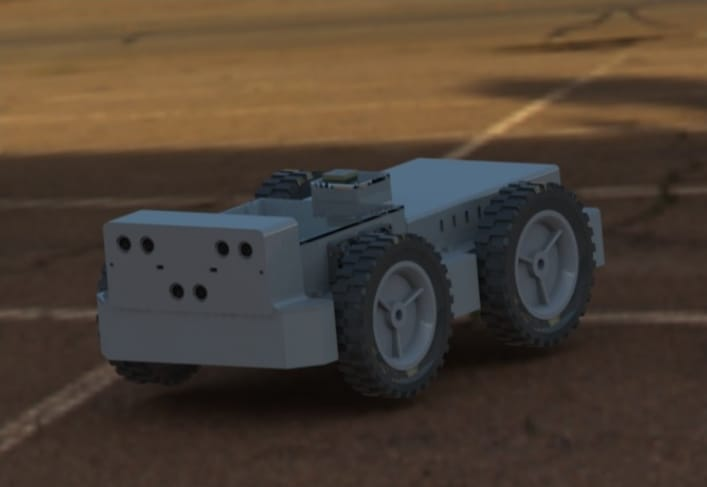
\includegraphics[width=0.5\textwidth]{imagens/projeto-fred.jpeg}
    
    {\small Fonte: Autoria própria}
\end{figure}

\begin{figure}[h]
    \centering
    \captionsetup{justification=centering}
    \caption{\small Equipe do projeto AMR Frederico}
    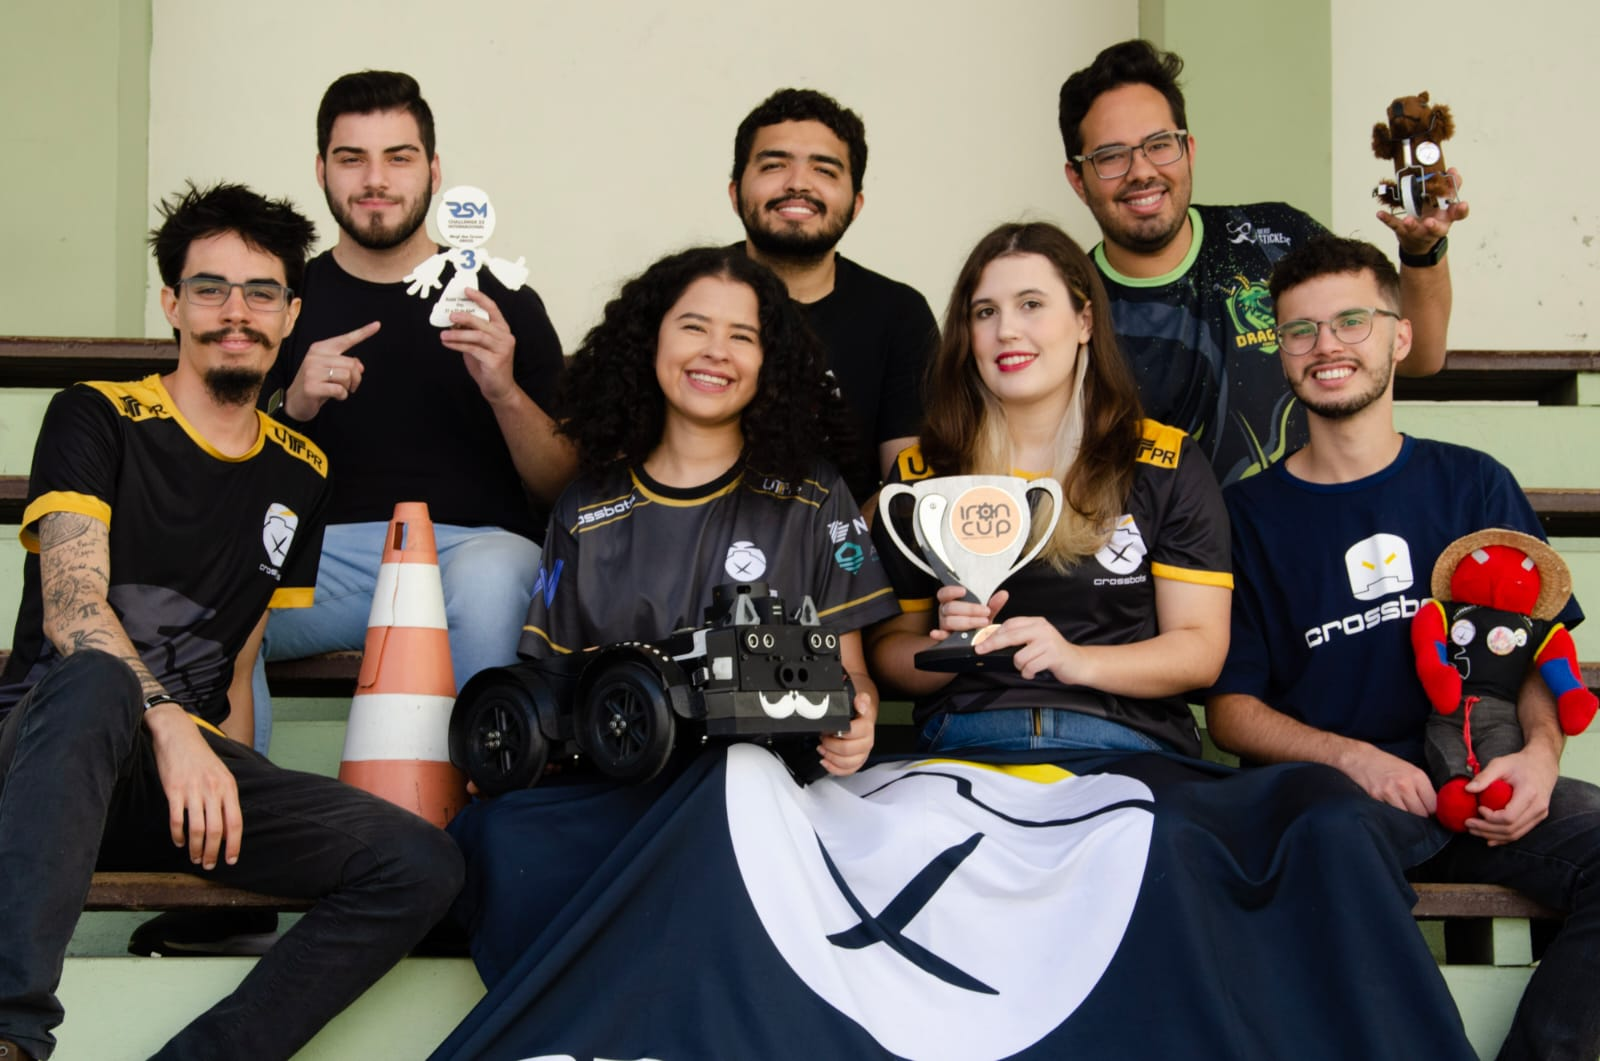
\includegraphics[width=0.5\textwidth]{imagens/TIme-fred.jpeg}
    
    {\small Fonte: Autoria própria}
\end{figure}

O Frederico é um AMR idealizado para robótica competitiva, na categoria \emph{Trekking Pro/Robomagellan}, cujo objetivo é "incentivar o desenvolvimento de veículos autônomos, utilizando as tecnologias mais avançadas nos campos de inteligência artificial, visão computacional, sensoriamento espacial, entre outras áreas da ciência"\cite{robocore}

A competição funciona da seguinte maneira, haverá 4 marcos (chapa de metal de cor amarela de dimensões aproximadas: 1000mm x 1000mm x 2mm.) posicionados aleatoriamente no ambiente de prova, o robô começa do marco 1 e deve chegar nos demais marcos — em ordem crescente — de forma autônoma, e entre o 3.º marco e o 4.º haverá obstáculos que o AMR deverá desviar. Ganha quem completar o circuito de forma mais rápida. Mais detalhes das regras poderão ser encontradas no Anexo XX.

\begin{figure}[h]
    \centering
    \captionsetup{justification=centering}
    \caption{\small Exemplo do campo de prova na competição de \emph{Trekking}}
    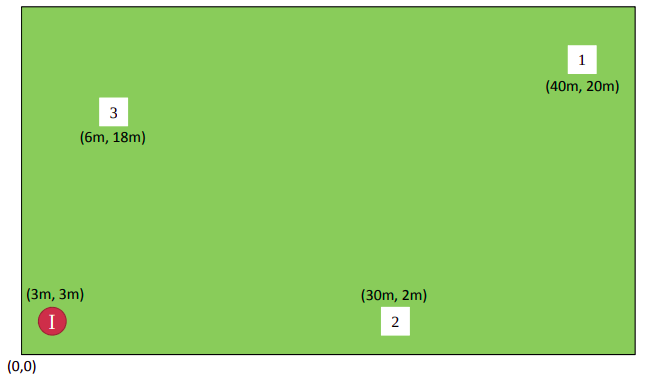
\includegraphics[width=0.5\textwidth]{imagens/ex-prova-trekking.png}
    
    {\small Fonte: \cite{robocore}}
\end{figure}

Discutiremos o processo de implementação do AMR Frederico, aspectos de projeto mecânico, \emph{hardware} e \emph{software}, integração dos sensores, odometria, mapeamento e principalmente seu sistema de navegação e ao final, os resultados obtidos do desempenho do robô. 

Esta pesquisa visa não apenas aperfeiçoar a performance do AMR Frederico, mas também contribuir para o avanço do conhecimento na área de robótica móvel autônoma, especialmente na aplicação de técnicas de controle para melhorar a navegação conhecidas, mas muitas vezes de difícil implementação.


% 1.2 ----------- problemas e premissas
\section{\textbf{Problemas e premissas}}

Nesta seção, exploraremos os desafios inerentes à navegação autônoma de robôs móveis e delinearemos as premissas que orientam nossa pesquisa. Compreender esses problemas e premissas é fundamental para estabelecer o contexto e a base subjacente deste trabalho.

A navegação autônoma de robôs móveis é uma tarefa complexa que enfrenta desafios significativos, porque a principal premissa para navegação é saber onde está no momento, onde fica o destino e como alcançá-lo \cite{Alatise2020}, em ambientes em constante mudança, onde a incerteza na percepção do ambiente e a imprecisão dos sensores podem impactar a qualidade da navegação. 

Além dos desafios de percepção e localização, a implementação de técnicas de controle robusto é essencial. Desenvolver algoritmos de controle capazes de garantir a estabilidade e eficácia da navegação autônoma é uma tarefa complexa devido à interação dinâmica entre o robô e o ambiente.

Para conduzir esta pesquisa, adotamos as seguintes premissas básicas:

\begin{itemize}
    \item \textbf{Implementação AMR Frederico:} Esta dissertação se concentrará na implementação do sistema de navegação no robô móvel autônomo Frederico. A pesquisa será orientada para alcançar melhorias específicas na navegação desse robô em ambientes não estruturados.
    \item \textbf{Utilização do \emph{Robot Operating System} (ROS):} A utilização do ROS vem com o intuito de utilizar ferramentas pensadas para robótica, e com isso, possuem uma série de ferramentas e bibliotecas que facilitam a implementação e integração de sistemas complexos. 
    \item \textbf{Implementação da navegação:} O sistema de navegação será implementado tendo como premissa as condições de prova da categoria \textit{Robomagellan/Trekking}.
    \item \textbf{Condições do ambiente:} O ambiente onde o robô Frederico operará é conhecido e mapeado, incluindo obstáculos estáticos e possivelmente dinâmicos.
\end{itemize}

A pesquisa abordará esses problemas, buscando desenvolver soluções que aprimorem as capacidades de navegação autônoma de robôs móveis. Além disso, a aplicação bem-sucedida dessas soluções tem o potencial de impactar positivamente várias áreas, incluindo logística, manufatura e serviços.

% 1.3 ----------- objetivos
\section{\textbf{Objetivos}}
Os objetivos deste trabalho estão centrados na implementação e aprimoramento do robô móvel autônomo AMR Frederico, para competições Trekking. Esses objetivos compreendem o desenvolvimento de diversas áreas, alinhando-se ao objetivo geral de criar um AMR eficiente, preciso e adaptável aos desafios das competições.

% 1.3.1 ---------- objetivo geral 
\subsection{Objetivo geral}
O objetivo geral deste trabalho é projetar, implementar o AMR Frederico para participação em competições Robomagellan. O foco principal é a implementação do robô como um sistema integrado, abordando desde a estrutura mecânica até o desenvolvimento de algoritmos de navegação.

O AMR Frederico será concebido para navegar autonomamente em ambientes desconhecidos, mapeando o cenário, evitando obstáculos e otimizando suas rotas. A implementação considerará a utilização de sensores, fusão de dados e utilização de filtros para que possamos ter um sistema de percepção confiável. Além disso, o uso da plataforma ROS será explorado para facilitar a integração e implementação de sistemas de sensoriamento, localização, mapeamento, navegação e locomoção.

Este objetivo geral envolve a realização de uma pesquisa aprofundada para compreender as necessidades da competição \textit{Robomagellan}, a análise das tecnologias disponíveis para navegação autônoma e a aplicação prática dessas tecnologias no projeto do Frederico. O robô resultante deverá ser capaz de realizar com sucesso as provas propostas pela competição, demonstrando sua eficiência e robustez em ambientes desafiadores e variados.

% 1.3.2 ---------- objetivos específicos
\subsection{Objetivos específicos}
Os objetivos específicos deste trabalho foram delineados para abordar aspectos cruciais da implementação e otimização do robô móvel autônomo Frederico:
\begin{itemize}
    \item \textbf{Seleção e integração de sensores:} Escolher e integrar sensores adequados para percepção do ambiente, localização e detecção de obstáculos.
    \item \textbf{Desenvolvimento de Software Embarcado:} Implementar o sistema operacional e \textit{softwares} necessários para controlar e coordenar os diferentes componentes do robô.
    \item \textbf{Algoritmos de Localização e Navegação:} Desenvolver algoritmos de localização que permitam que o robô determine sua posição em relação ao ambiente. Implementar algoritmos de navegação que permitam ao Frederico traçar rotas evitando obstáculos e cumprindo os objetivos da competição.
    \item \textbf{Integração de Sistemas via ROS:} Explorar a plataforma ROS para integrar de maneira eficiente os diferentes sistemas e subsistemas do robô, simplificando o desenvolvimento e testes.
    \item \textbf{Preparação para Competições:} Adaptar o Frederico às condições específicas das competições \textit{Robomagellan}, garantindo que ele seja capaz de cumprir as tarefas propostas, como localização de pontos e navegação em cenários desconhecidos.
    \item \textbf{Análise e Resultados:} Analisar os resultados dos testes e competições, avaliando o desempenho do robô em relação aos objetivos estabelecidos. Identificar áreas de melhoria e propor possíveis ajustes.
\end{itemize}

Essas metas serão abordados ao longo deste trabalho, fornecendo uma visão abrangente e detalhada do processo de implementação e aplicação do robô móvel autônomo Frederico em competições \textit{Trekking}.


% 1.4 ------------ justificativa 
\section{\textbf{Justificativa}}

A justificativa para este trabalho se fundamenta na importância da navegação natural em robôs móveis autônomos e na necessidade de soluções eficientes que possam ser aplicadas em diversos setores. Enquanto as abordagens tradicionais de navegação muitas vezes enfrentam limitações ao lidar com ambientes desconhecidos, a implementação da navegação natural apresenta um potencial impacto positivo, permitindo que os robôs se movam de forma autônoma e eficaz em ambientes complexos e dinâmicos.

A relevância deste trabalho é acentuada pela contribuição do projeto Frederico, que se concentra na pesquisa em robótica móvel autônoma e na preparação para a competição de \textit{Trekking}. O projeto aborda desafios reais de navegação e exploração, oferecendo uma oportunidade para o desenvolvimento e aprimoramento de sistemas de percepção, localização, controle e planejamento de trajetória.

Ao aplicar a navegação natural no robô Frederico, não apenas demonstramos a viabilidade da tecnologia em situações práticas, mas também contribuímos para o avanço da pesquisa científica na área de robótica. Além disso, ao participar de competições como Robomagellan, estamos promovendo a inovação e a busca por soluções eficientes, ao mesmo tempo em que inspiramos futuras aplicações em cenários industriais e de serviços.

% 1.5 ------------ estrutura do trabalho
\section{\textbf{Estrutura do trabalho}}

Este trabalho segue uma organização em capítulos, cada um com um propósito específico para alcançar os objetivos gerais do projeto. Uma breve visão geral de cada capítulo é apresentada a seguir:

Capítulo 2: Revisão Bibliográfica
Este capítulo é dedicado a uma revisão abrangente da literatura relacionada à navegação natural em robôs móveis autônomos. Serão abordadas questões relevantes, como técnicas de localização e mapeamento simultâneos (SLAM), estratégias de planejamento de trajetória, tipos de sensores empregados na navegação e sistemas de controle utilizados. Essa revisão literária fornecerá um contexto sólido para compreender as abordagens atuais e os avanços na área.

Capítulo 3: Metodologia
Este capítulo explora as metodologias empregadas no desenvolvimento do projeto Frederico. Detalhes sobre os componentes de hardware e software selecionados, incluindo sensores e \textit{softwares} utilizados, serão apresentados. Além disso, abordaremos a montagem e configuração do robô. 

Capítulo 4: Testes e Resultados
Neste capítulo, apresentaremos os resultados obtidos após a implementação da navegação natural no AMR Frederico. Analisaremos e discutiremos os dados coletados durante os testes, destacando tanto os sucessos quanto os desafios enfrentados durante o processo. Também discutiremos as soluções desenvolvidas para superar obstáculos e otimizar o desempenho do robô.

Capítulo 5: Considerações finais
No último capítulo, faremos uma síntese das principais conclusões derivadas deste trabalho. Revisitaremos os objetivos alcançados e suas implicações, além de discutir as contribuições significativas para a pesquisa em navegação natural em robôs móveis autônomos. Abordaremos também as limitações encontradas e sugeriremos possíveis direções para futuras investigações nesse campo.

Referências Bibliográficas e Anexos:
E por fim, nos dois últimos capítulos contém fontes e referências bibliográficas consultadas ao longo deste trabalho e demais materias nos anexos que foram fundamentais para a realização desta pesquisa e/ou compreensão do leitor. 
